\documentclass[aspectratio=169]{beamertmd}

\usepackage{amsmath}
\usepackage{amssymb}
\usepackage{wasysym}
\usepackage{graphicx}
\usepackage{tikz}

\title{Wave-Based Modeling for Jointed Structures}
\author{Nidish Narayanaa Balaji}

\AtBeginSection[]{\frame{\sectionpage{}}}

\begin{document}
\maketitle{}

\begin{frame}
  \frametitle{Outline}
  \tableofcontents{}
\end{frame}

\section{Governing Equations and System of Interest}
\label{sec:govern-equat-syst}

\begin{frame}[allowframebreaks]
  \frametitle{Dispersion of the Timoshenko Beam}
  \vspace{-0.5cm}\begin{figure}[!h]
    \centering
    \includegraphics[height=2cm]{FIGS/CSYS}
  \end{figure}      
  \begin{itemize}
  \item The coordinate systems that will be used here are given in the
    figure above. The beam is taken to be in the XY plane and the
    degrees of freedom for each point on the beam are taken to be
    the displacements $u_x$, $u_y$, and rotation $\theta_z$.
  \item The equations of motion used for the Timoshenko beam are:
    {\tiny
      \begin{align*}
        \begin{bmatrix} \rho A & 0 & 0\\ 0 & \rho A & 0\\0 & 0 & \rho
          I_z \end{bmatrix} \frac{\partial^2}{\partial
                                                                 t^2}\begin{Bmatrix}
                                                                 u_x\\
                                                                 u_y\\\theta_z \end{Bmatrix}
        - \begin{bmatrix} EA & 0 & 0\\ 0 & GA & 0\\0 & 0 &
          EI_z \end{bmatrix} \frac{\partial^2}{\partial
                                                           x^2} \begin{Bmatrix}
                                                           u_x\\u_y\\\theta_z \end{Bmatrix}
        + \begin{bmatrix} 0 & 0 & 0\\ 0 & 0 & GA \\ 0 & -GA &
          0 \end{bmatrix} \frac{\partial}{\partial x}\begin{Bmatrix}
          u_x\\u_y\\\theta_z \end{Bmatrix} + \begin{bmatrix} 0 & 0 & 0
          \\ 0 & 0 & 0 \\ 0 & 0 & GA \end{bmatrix} \begin{Bmatrix}
          u_x\\ u_y\\\theta_z \end{Bmatrix} = \begin{Bmatrix} f_x\\
          f_y\\ m_z\end{Bmatrix}. 
      \end{align*}}
    \pagebreak
  \item Dispersion relationships will be discussed using the wave
    representation $\bar{u} = \bar{U} e^{i(k x-\omega t)}$. 
  \item The dispersion relationship for the axial vibration
    (longitudinal waves) is
    $$ \omega = \sqrt{\frac{E}{\rho}} k $$
  \item For bending vibration (transverse waves), the dispersion
    relationship is
    $$ (\rho^2AI_z)\omega^4 - \left[\rho GA^2+k^2\rho
      AI_z(G+E)\right] \omega^2 + (EGAI_z) k^4 = 0 $$
    \pagebreak
  \item The dispersion relationship is presented below graphically for
    a case corresponding to $E=200 GPa$, $\nu=0.3$, $\rho=7800 kg
    m^{-3}$ and a square cross-section of $25.4 mm$.
    \vspace{-0.5cm}
    \begin{figure}[!h]
      \centering
      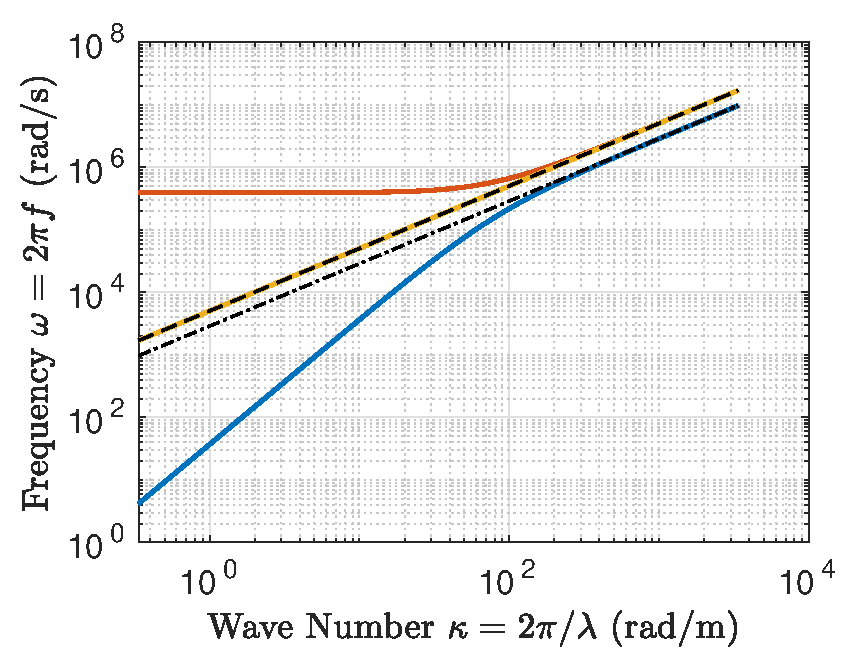
\includegraphics[width=0.35\linewidth]{../../PLANARMODEL/FIGS/TMWS_WvK}%
      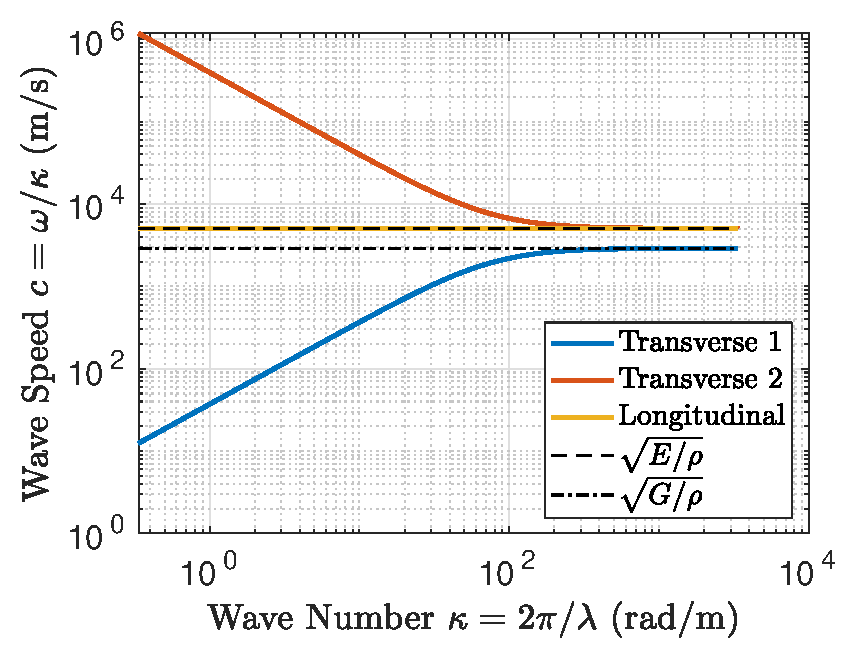
\includegraphics[width=0.35\linewidth]{../../PLANARMODEL/FIGS/TMWS_CvK}%
      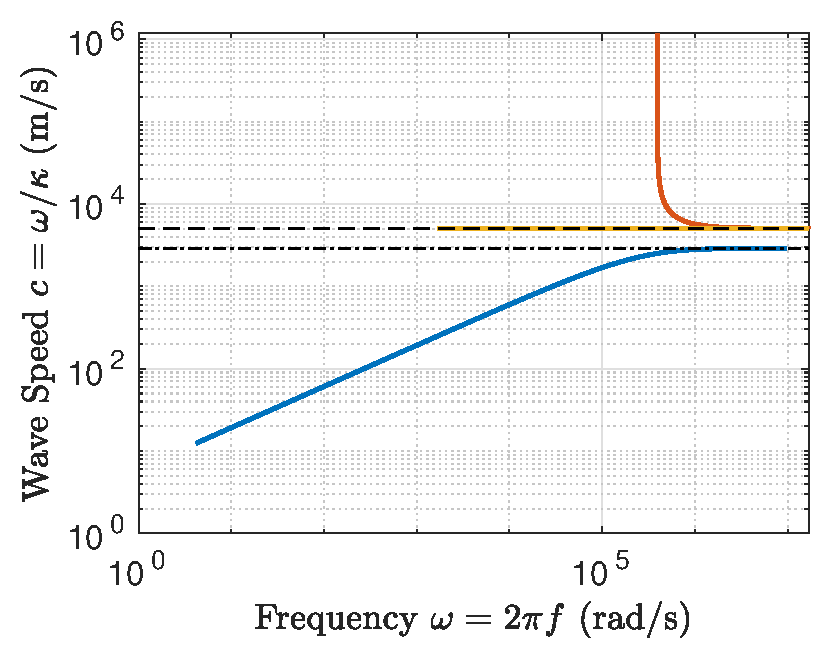
\includegraphics[width=0.35\linewidth]{../../PLANARMODEL/FIGS/TMWS_CvW}
    \end{figure}
  \item Asymptotes corresponding to the case $\omega\to \infty$ are
    depicted using dashed lines in the figure
  \end{itemize}
\end{frame}

\begin{frame}[allowframebreaks]
  \frametitle{Brake-Reu{\ss} Beam Benchmark}
  \begin{itemize}
  \item The following is a schematic representation of the
    Brake-Reu{\ss} Beam (BRB) benchmark that the techniques will be
    applied to first. All dimensions are in mm and the in-plane
    thickness is also 25.4 mm.
    \begin{figure}[!h]
      \centering
      \includegraphics[width=0.8\linewidth]{../../PLANARMODEL/FIGS/brbdesign}
    \end{figure}
  \item The interface region is discretized using 4, 8, 16, and 32
    elements to study the influence of mesh density.
  \item The bolt prestress is modeled by simulating a normal pressure
    distribution described by a sum of three Gaussian distributions
    with means at equidistant locations and standard deviations
    equal to 10.265 mm (fixed through washer dimensions and 33 degree
    pressure cone).
  \item The following shows the ``bolt-traction'' distribution and the
    static prestress solution of the system.
    \pagebreak
    \begin{figure}[!h]
      \centering
      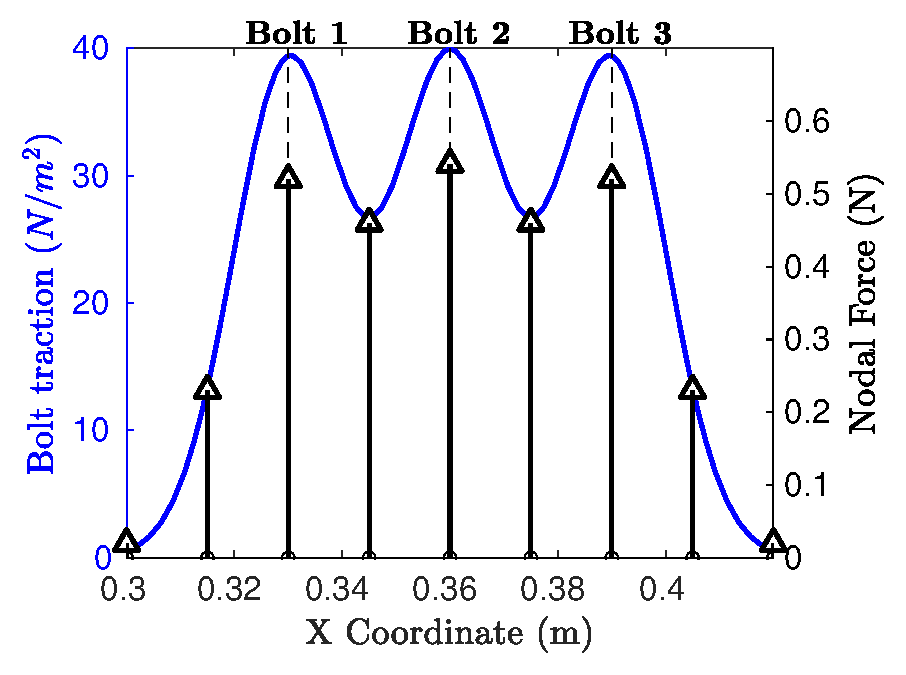
\includegraphics[width=0.5\linewidth]{../../PLANARMODEL/FIGS/BOLTFORCMOD_8IN}%
      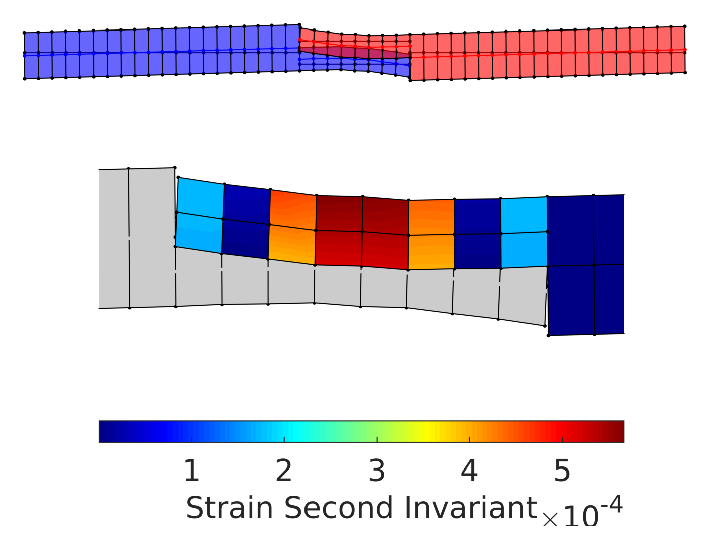
\includegraphics[width=0.5\linewidth]{../../PLANARMODEL/FIGS/8IN_PRESSOL}
      \caption{Bolt traction distribution and Static Prestress
        solution (displacements magnified 500x). The second strain
        invariant is $(\sigma_1^2+\sigma_2^2)/2$.}
    \end{figure}
    \pagebreak
  \item The first five modal frequencies and mode shapes of this
    structure are given here
    \begin{columns}
      \begin{column}{0.5\linewidth}
        \begin{table}[!h]
          \centering
          \begin{tabular}{cc}
            \hline\hline
            Sno. & Natural Frequency (Hz)\\\hline
            1 & 265.10\\
            2 & 691.79\\
            3 & 1384.91\\
            4 & 2165.98\\
            5 & 3057.76\\\hline\hline
          \end{tabular}
          \caption{First Five Natural Frequencies}
        \end{table}
      \end{column}
      \begin{column}{0.5\linewidth}
        \begin{figure}[!h]
          \centering
          \includegraphics[width=\linewidth]{../../PLANARMODEL/FIGS/8IN_PRESLINMDS}
        \end{figure}
      \end{column}
    \end{columns}
    \pagebreak
  \item Below the natural frequencies are plotted against the
    Dispersion plot:
    \begin{figure}[!h]
      \centering
      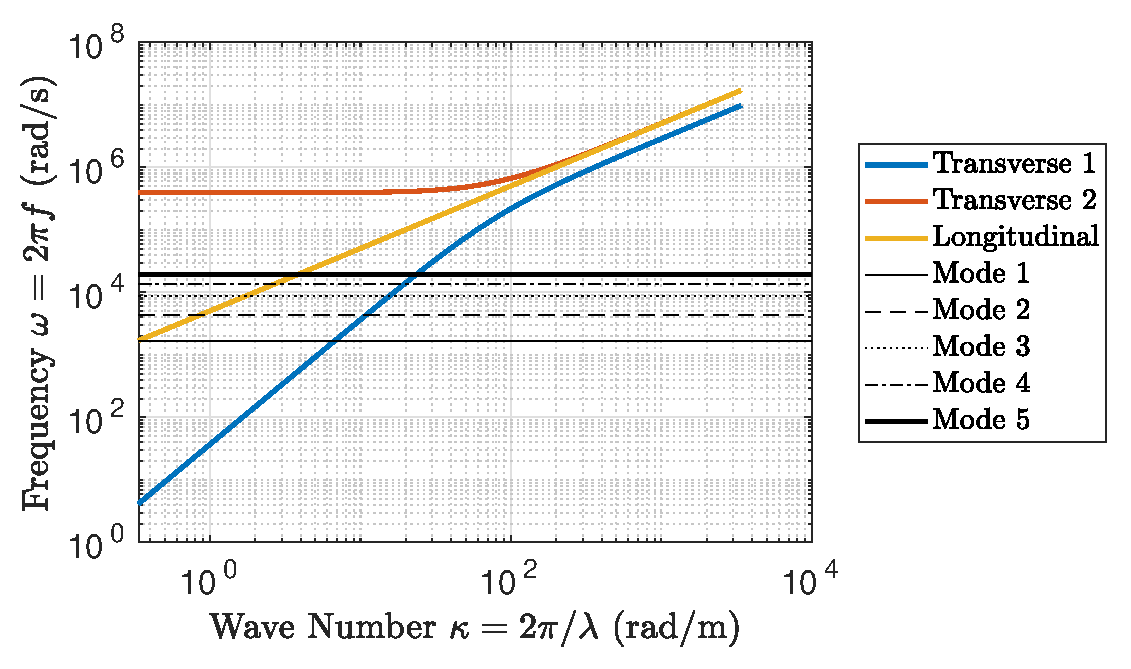
\includegraphics[width=0.6\linewidth]{../../PLANARMODEL/FIGS/TMWS_WvK_wmf}
    \end{figure}
  \item \underline{Observation}: The second transverse wave does not 
    seem to be engaged in the first five modes that might be
    interesting later on.
  \end{itemize}
\end{frame}

\begin{frame}[allowframebreaks]
  \frametitle{Wave Propagation Calculations}
  \framesubtitle{Longitudinal Waves}
  \begin{block}{Equations of Motion}
    {\tiny
      \begin{align*}
        \begin{bmatrix} \rho A & 0 & 0\\ 0 & \rho A & 0\\0 & 0 & \rho
          I_z \end{bmatrix} \frac{\partial^2}{\partial
                                                                 t^2}\begin{Bmatrix}
                                                                 u_x\\
                                                                 u_y\\\theta_z \end{Bmatrix}
        - \begin{bmatrix} EA & 0 & 0\\ 0 & GA & 0\\0 & 0 &
          EI_z \end{bmatrix} \frac{\partial^2}{\partial
                                                           x^2} \begin{Bmatrix}
                                                           u_x\\u_y\\\theta_z \end{Bmatrix}
        + \begin{bmatrix} 0 & 0 & 0\\ 0 & 0 & GA \\ 0 & -GA &
          0 \end{bmatrix} \frac{\partial}{\partial x}\begin{Bmatrix}
          u_x\\u_y\\\theta_z \end{Bmatrix} + \begin{bmatrix} 0 & 0 & 0
          \\ 0 & 0 & 0 \\ 0 & 0 & GA \end{bmatrix} \begin{Bmatrix}
          u_x\\ u_y\\\theta_z \end{Bmatrix} = \begin{Bmatrix} f_x\\
          f_y\\ m_z\end{Bmatrix}. 
      \end{align*}}
  \end{block}
  \begin{itemize}
  \item Longitudinal waves are decoupled from transverse waves and are
    therefore considered separately.
  \item Choosing the symbol $a_\ell^+$ and $a_\ell^-$ to denote complex
    amplitudes of forward and backward propagating waves, the
    longitudinal-only solution to the equations is:
    $$ u_x(x, t) = a_\ell^+ e^{-i(k_\ell x-\omega t)} + a_\ell^-
    e^{i(k_\ell x+\omega t)}. $$
  \item The dispersion relationship for $k_\ell$ and $\omega$ is,
    $$ \omega^2 = \underbrace{\frac{E}{\rho}}_{C_\ell^2} k_\ell^2. $$
  \item The wave-speed $C_\ell=\sqrt{\frac{E}{\rho}}$ is a constant
    for this case.
  \item Considering two points $x_A$ and $x_B$ on the beam with wave
    amplitudes $a_\ell^\pm$ and $b_\ell^\pm$ respectively, the
    following propagation relationship may be written for a fully
    linear beam:
    $$ b_{\ell}^+ = e^{-ik_{\ell}(x_A-x_B)} a_{\ell}^+\qquad
    b_{\ell}^- = e^{ik_{\ell}(x_A-x_B)} a_{\ell}^- $$
  \end{itemize}
\end{frame}

\begin{frame}[allowframebreaks]
  \frametitle{Wave Propagation Calculations}
  \framesubtitle{Transverse Waves}
  \begin{block}{Equations of Motion}
    {\tiny
      \begin{align*}
        \begin{bmatrix} \rho A & 0 & 0\\ 0 & \rho A & 0\\0 & 0 & \rho
          I_z \end{bmatrix} \frac{\partial^2}{\partial
                                                                 t^2}\begin{Bmatrix}
                                                                 u_x\\
                                                                 u_y\\\theta_z \end{Bmatrix}
        - \begin{bmatrix} EA & 0 & 0\\ 0 & GA & 0\\0 & 0 &
          EI_z \end{bmatrix} \frac{\partial^2}{\partial
                                                           x^2} \begin{Bmatrix}
                                                           u_x\\u_y\\\theta_z \end{Bmatrix}
        + \begin{bmatrix} 0 & 0 & 0\\ 0 & 0 & GA \\ 0 & -GA &
          0 \end{bmatrix} \frac{\partial}{\partial x}\begin{Bmatrix}
          u_x\\u_y\\\theta_z \end{Bmatrix} + \begin{bmatrix} 0 & 0 & 0
          \\ 0 & 0 & 0 \\ 0 & 0 & GA \end{bmatrix} \begin{Bmatrix}
          u_x\\ u_y\\\theta_z \end{Bmatrix} = \begin{Bmatrix} f_x\\
          f_y\\ m_z\end{Bmatrix}. 
      \end{align*}}
  \end{block}
  \begin{itemize}
  \item Transverse waves are studied independent of longitudinal waves
    since the equations are naturally decoupled (for the linear case)
  \item From theory (see Mei and Mace, 2005) and the wave speed plots
    before, it is known that two waves exist for transverse vibrations
    of Timoshenko beams
  \item The wave numbers of these are denoted as $k_1$ and $-i k_2$
    respectively.
  \item The second wave is not harmonic unless the frequency is above
    a critical cut-off.
  \item The cut-off is found by evaluating the solution of the
    dispersion relationship in the limit $k\to 0$ as follows:
    \begin{align*}
      \omega^2 \left[ (\rho^2AI_z)\omega^2 - (\rho GA^2)\right] &= 0\\
      \implies \omega = \underbrace{0, 0}_{\text{first kind}}
      \quad;\quad &\underbrace{\sqrt{\frac{GA}{\rho I_z}},
                    -\sqrt{\frac{GA}{\rho I_z}}}_{\text{second kind}}\\
      \text{denote } \omega_c = \sqrt{\frac{GA}{\rho I_z}}.
    \end{align*}
  \item For frequencies $\omega<\omega_c$, the waves of the second
    kind occur as pairs of growing and decaying components. The
    current study will be restricted to this region. 
  \item In these cases, the wave number will be complex and therefore
    $-i k_2$ is used to denote the wave number of convenience.
  \item With forward and backward components for each kinds of waves
    $a_1^\pm$, $a_2^\pm$, the transverse displacement is represented as,
    \begin{align*}
      u_y(x, t) &= \underbrace{a_1^+e^{-i(k_1x-\omega t)} +
                  a_1^-e^{i(k_1x+\omega t)}}_{\text{first kind waves}} +
                  \underbrace{a_2^+e^{-(k_2x-i\omega t)} + a_2^-e^{(k_2x+i\omega
                  t)}}_{\text{second kind waves}}
    \end{align*}
  \item Similarly, with amplitudes $\overline{a_1^\pm}$,
    $\overline{a_2^\pm}$, the rotations are written as,
    \begin{align*}
      \theta_z(x, t) &= \underbrace{\overline{a_1^+} e^{-i(k_1x-\omega t)}
                       + \overline{a_1^-} e^{i(k_1x+\omega
                       t)}}_{\text{first kind waves}} +
                       \underbrace{\overline{a_2^+} e^{-(k_2x-i\omega t)} +
                       \overline{a_2^-} e^{(k_2x+i\omega t)}}_{\text{second
                       kind waves}} 
    \end{align*}
  \item Substituting these back into the equations of motions allows
    one to obtain relationships between $a_{1,2}^\pm$ and
    $\overline{a_{1,2}}^\pm$:
    \begin{itemize}
    \item For ($a_1^+$, $\overline{a_1^+}$),
      \begin{align*}
        \begin{bmatrix} (GA)k_1^2-(\rho A)\omega^2 & -ik_1(GA)\\
          ik_1(GA) & (EI_z)k_1^2-(\rho I_z)\omega^2
          (GA) \end{bmatrix} \begin{Bmatrix} a_1^+\\
          \overline{a_1^+} \end{Bmatrix} = \begin{Bmatrix} 0\\
          0 \end{Bmatrix}.\\
        \implies \boxed{\frac{a_1^+}{\overline{a_1^+}} =
        -ik_1\left(1-\frac{\omega^2}{C_s^2k_1^2}\right)} \quad
        \text{with } C_s^2 = \frac{G}{A}.
      \end{align*}        
    \item For ($a_1^-$, $\overline{a_1^-}$),
      \begin{align*}
        \begin{bmatrix} (GA)k_1^2-(\rho A)\omega^2 & ik_1(GA)\\
          -ik_1(GA) & (EI_z)k_1^2-(\rho I_z)\omega^2
          (GA) \end{bmatrix} \begin{Bmatrix} a_1^-\\
          \overline{a_1^-} \end{Bmatrix} = \begin{Bmatrix} 0\\
          0 \end{Bmatrix}.\\
        \implies \boxed{\frac{a_1^-}{\overline{a_1^-}} =
        ik_1\left(1-\frac{\omega^2}{C_s^2k_1^2}\right)}. 
      \end{align*}
    \item For ($a_2^+$, $\overline{a_2^+}$),
      \begin{align*}
        \begin{bmatrix} -(GA)k_2^2-(\rho A)\omega^2 & -k_2(GA)\\
          k_2(GA) & -(EI_z)k_2^2-(\rho I_z)\omega^2
          (GA) \end{bmatrix} \begin{Bmatrix} a_2^+\\
          \overline{a_2^+} \end{Bmatrix} = \begin{Bmatrix} 0\\
          0 \end{Bmatrix}.\\
        \implies \boxed{\frac{a_2^+}{\overline{a_2^+}} =
        -k_2\left(1+\frac{\omega^2}{C_s^2k_2^2}\right)}.
      \end{align*}
    \item For ($a_2^-$, $\overline{a_2^-}$),
      \begin{align*}
        \begin{bmatrix} -(GA)k_2^2-(\rho A)\omega^2 & k_2(GA)\\
          -k_2(GA) & -(EI_z)k_2^2-(\rho I_z)\omega^2
          (GA) \end{bmatrix} \begin{Bmatrix} a_2^-\\
          \overline{a_2^-} \end{Bmatrix} = \begin{Bmatrix} 0\\
          0 \end{Bmatrix}.\\
        \implies \boxed{\frac{a_2^-}{\overline{a_2^-}} =
        k_2\left(1+\frac{\omega^2}{C_s^2k_2^2}\right)}.
      \end{align*}
    \end{itemize}
  \item In summary we have,
    \begin{align*}
      \boxed{\frac{a_1^+}{\overline{a_1^+}} = -iP} \quad
      \boxed{\frac{a_1^-}{\overline{a_1^-}} = iP} \quad
      \boxed{\frac{a_2^+}{\overline{a_2^+}} = -N} \quad
      \boxed{\frac{a_2^-}{\overline{a_2^-}} = N}\\
      \text{with, } P =
      k_1\left(1-\frac{\omega^2}{C_s^2k_1^2}\right) \qquad N =
      k_2\left(1+\frac{\omega^2}{C_s^2k_2^2}\right).
    \end{align*}
  \item Substituting the above, we can express a general wave solution
    as, 
    {\footnotesize
      \begin{align*}
        \begin{Bmatrix} u_y\\ \theta_z \end{Bmatrix} = \begin{bmatrix}
          e^{-i(k_1x-\omega t)} & 
          e^{-(k_2x-i\omega t)} \\
          -(iP)e^{-i(k_1x-\omega t)} & -(N)
          e^{-(k_2x-i\omega t)} \end{bmatrix} \begin{Bmatrix} a_1^+\\
          a_2^+ \end{Bmatrix} + \begin{bmatrix} e^{i(k_1x+\omega t)} & 
          e^{(k_2x+i\omega t)}\\ (iP) e^{i(k_1x+\omega t)} & (N) e^{(k_2x+i\omega
            t)} \end{bmatrix} \begin{Bmatrix} a_1^-\\
          a_2^- \end{Bmatrix}
      \end{align*}}
  \item Considering points at $x_A$, $x_B$, with wave amplitudes
    $a_{1,2}^\pm$ and $b_{1,2}^\pm$ respectively, the propagation of
    the wave amplitudes may be written as,
    \begin{align*}
      \boxed{\begin{Bmatrix} b_1^+\\ b_2^+ \end{Bmatrix}
      = \begin{bmatrix} e^{-ik_1(x_A-x_B)} & 0\\0 &
        e^{-k_2(x_A-x_B)} \end{bmatrix} \begin{Bmatrix} a_1^+\\
          a_2^+ \end{Bmatrix}}\\
      \boxed{\begin{Bmatrix} b_1^-\\ b_2^- \end{Bmatrix}
      = \begin{bmatrix} e^{ik_1(x_A-x_B)} & 0\\0 &
        e^{k_2(x_A-x_B)} \end{bmatrix} \begin{Bmatrix} a_1^-\\
        a_2^- \end{Bmatrix}}
    \end{align*}
  \end{itemize}
\end{frame}

\section{Numerical Wave-based Study Methodology}
\label{sec:numerical-wave-based}

\subsection{Approach 1: Inhomogeneous Response}
\label{sec:appr-1:-inhom}

\begin{frame}[allowframebreaks]
  \frametitle{Numerical Wave-based Study Methodology}
  \framesubtitle{Approach 1: Inhomogeneous Response}
  \begin{itemize}
  \item Since an analytical solution does not exist for this problem,
    the study will be conducted using finite element simulations
  \item 1D linear Timoshenko beam elements are used for this purpose
  \item Force pulses are generated by windowing sines with a Hanning 
    window. An example is provided in the following slide.
  \item The width of the pulse will be chosen based on the size of the
    domain used for simulations.
  \item Simulations will be carried out for \emph{pulse frequencies}
    (frequency of the excitation pulse) ranging from 150 Hz up to 350
    Hz, so as to cover the first bending mode. 
    \pagebreak
    \begin{figure}[!h]
      \centering
      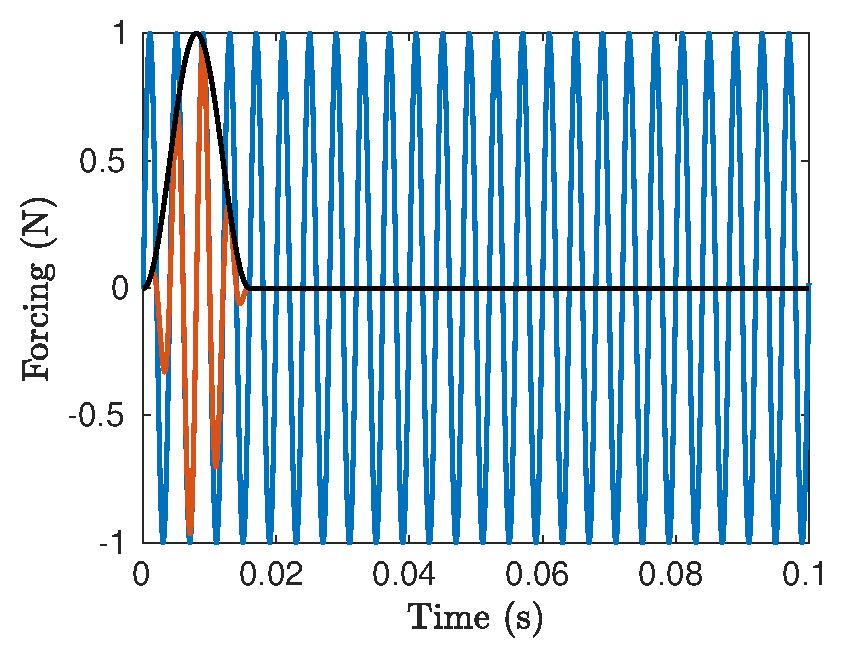
\includegraphics[width=0.5\linewidth]{../../PLANARMODEL/FIGS/HNWSIG_T}%
      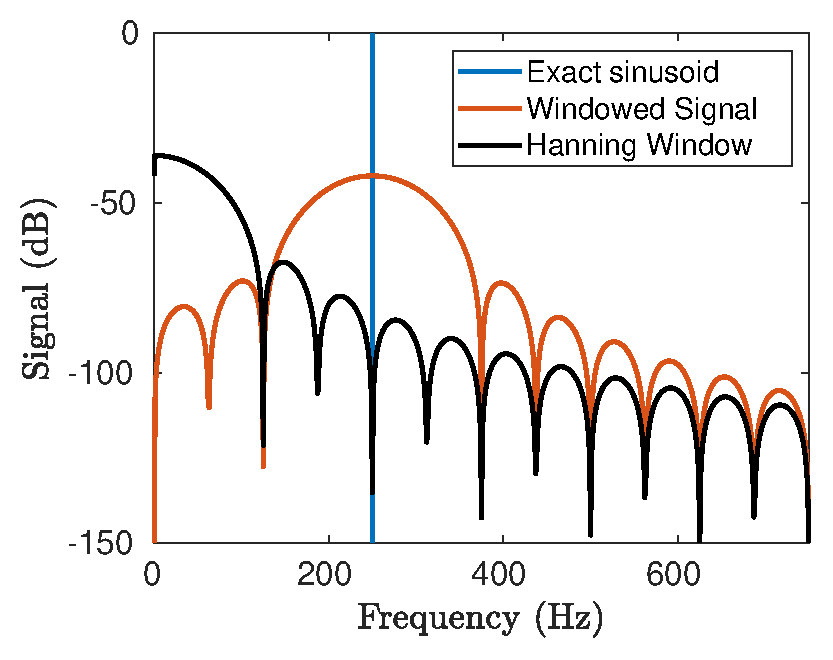
\includegraphics[width=0.5\linewidth]{../../PLANARMODEL/FIGS/HNWSIG_F}
      \caption{An exact sinusoid, }
    \end{figure}
    \pagebreak
  \item Using the dispersion relationships, the wave numbers,
    wavelengths, phase speeds and group speeds for the (transverse 1,
    transverse 2, longitudinal) waves are presented in parenthesis (in
    that order).
    \begin{table}[!h]
      \centering
      {\tiny
        \begin{tabular}{ccccc}
          \hline\hline\\
          Frequency (Hz) & Wavenumber (rad/m) & Wavelength (m) & Phase Speed (m/s) & Group Speed (m/s)\\\hline\\
          150.00 & (5.04, NaN, 0.19) &  (1.25, NaN, 33.76) &  (186.79, NaN, 5063.70) & (-1892.33, NaN, 5063.70)\\\\
          350.00 & (7.72, NaN, 0.43) &  (0.81, NaN, 14.47) & (284.82, NaN, 5063.70) &  (-4444.42, NaN, 5063.70)\\\hline\hline
        \end{tabular}}
    \end{table}
  \item By conducting time-frequency analyses of the response at
    specific locations along the beam, it is possible to build
    transmissibility matrices for pulses.
  \item A drawback here is that the different wave components in the
    transverse direction can not be distinguished using just
    time-frequency analysis.
    \pagebreak
  \item The following is the setup (left) and a sample response (DOF 1, 2, 3
    : $u_x, u_y, \theta_z$). 
    \begin{figure}
      \centering
      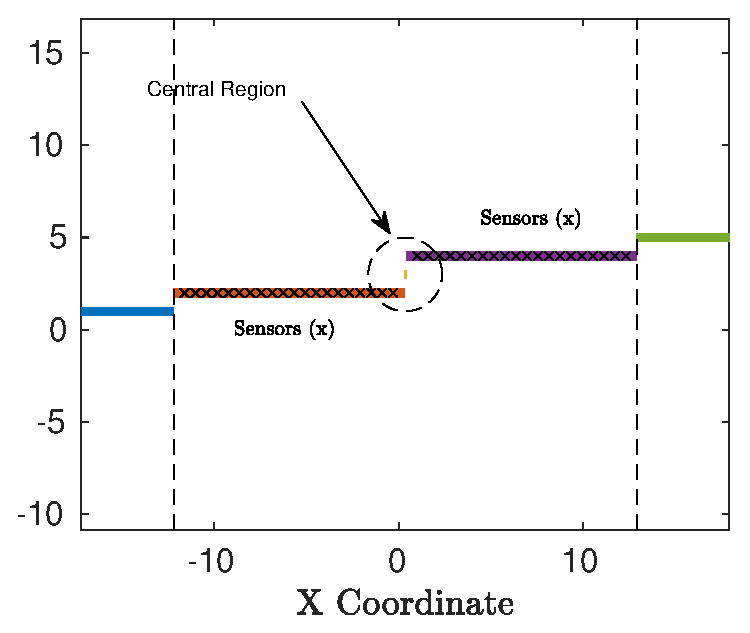
\includegraphics[width=0.5\linewidth]{../../PLANARMODEL/FIGS/FPULS_setupsamp}%
      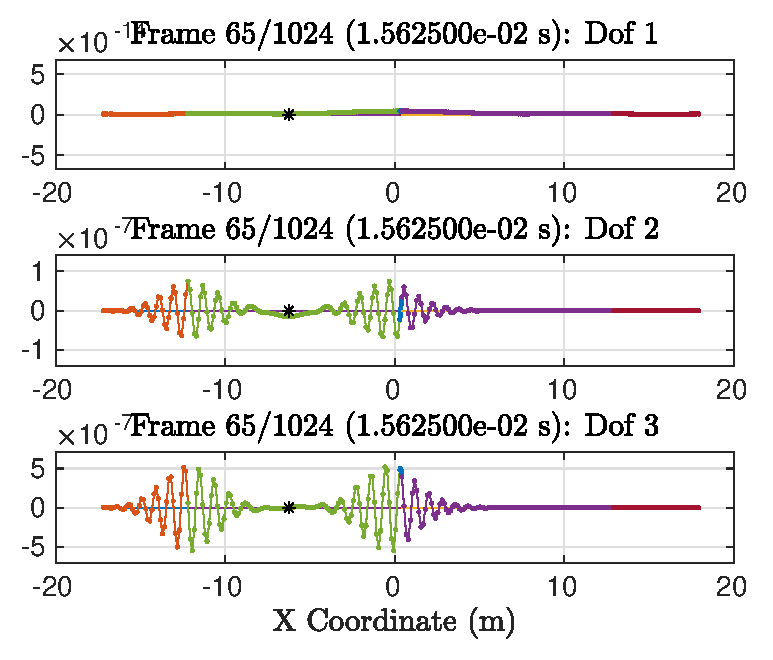
\includegraphics[width=0.5\linewidth]{../../PLANARMODEL/FIGS/FPULSERESP_samp}
    \end{figure}
  \item The forcing location is indicated with $*$ in the plots in the
    right.
    \pagebreak
  \item A time frequency analysis is conducted on 10 ``sensor
    locations'' along each beam regions (red and purple in previous slide):
    \begin{figure}
      \centering
      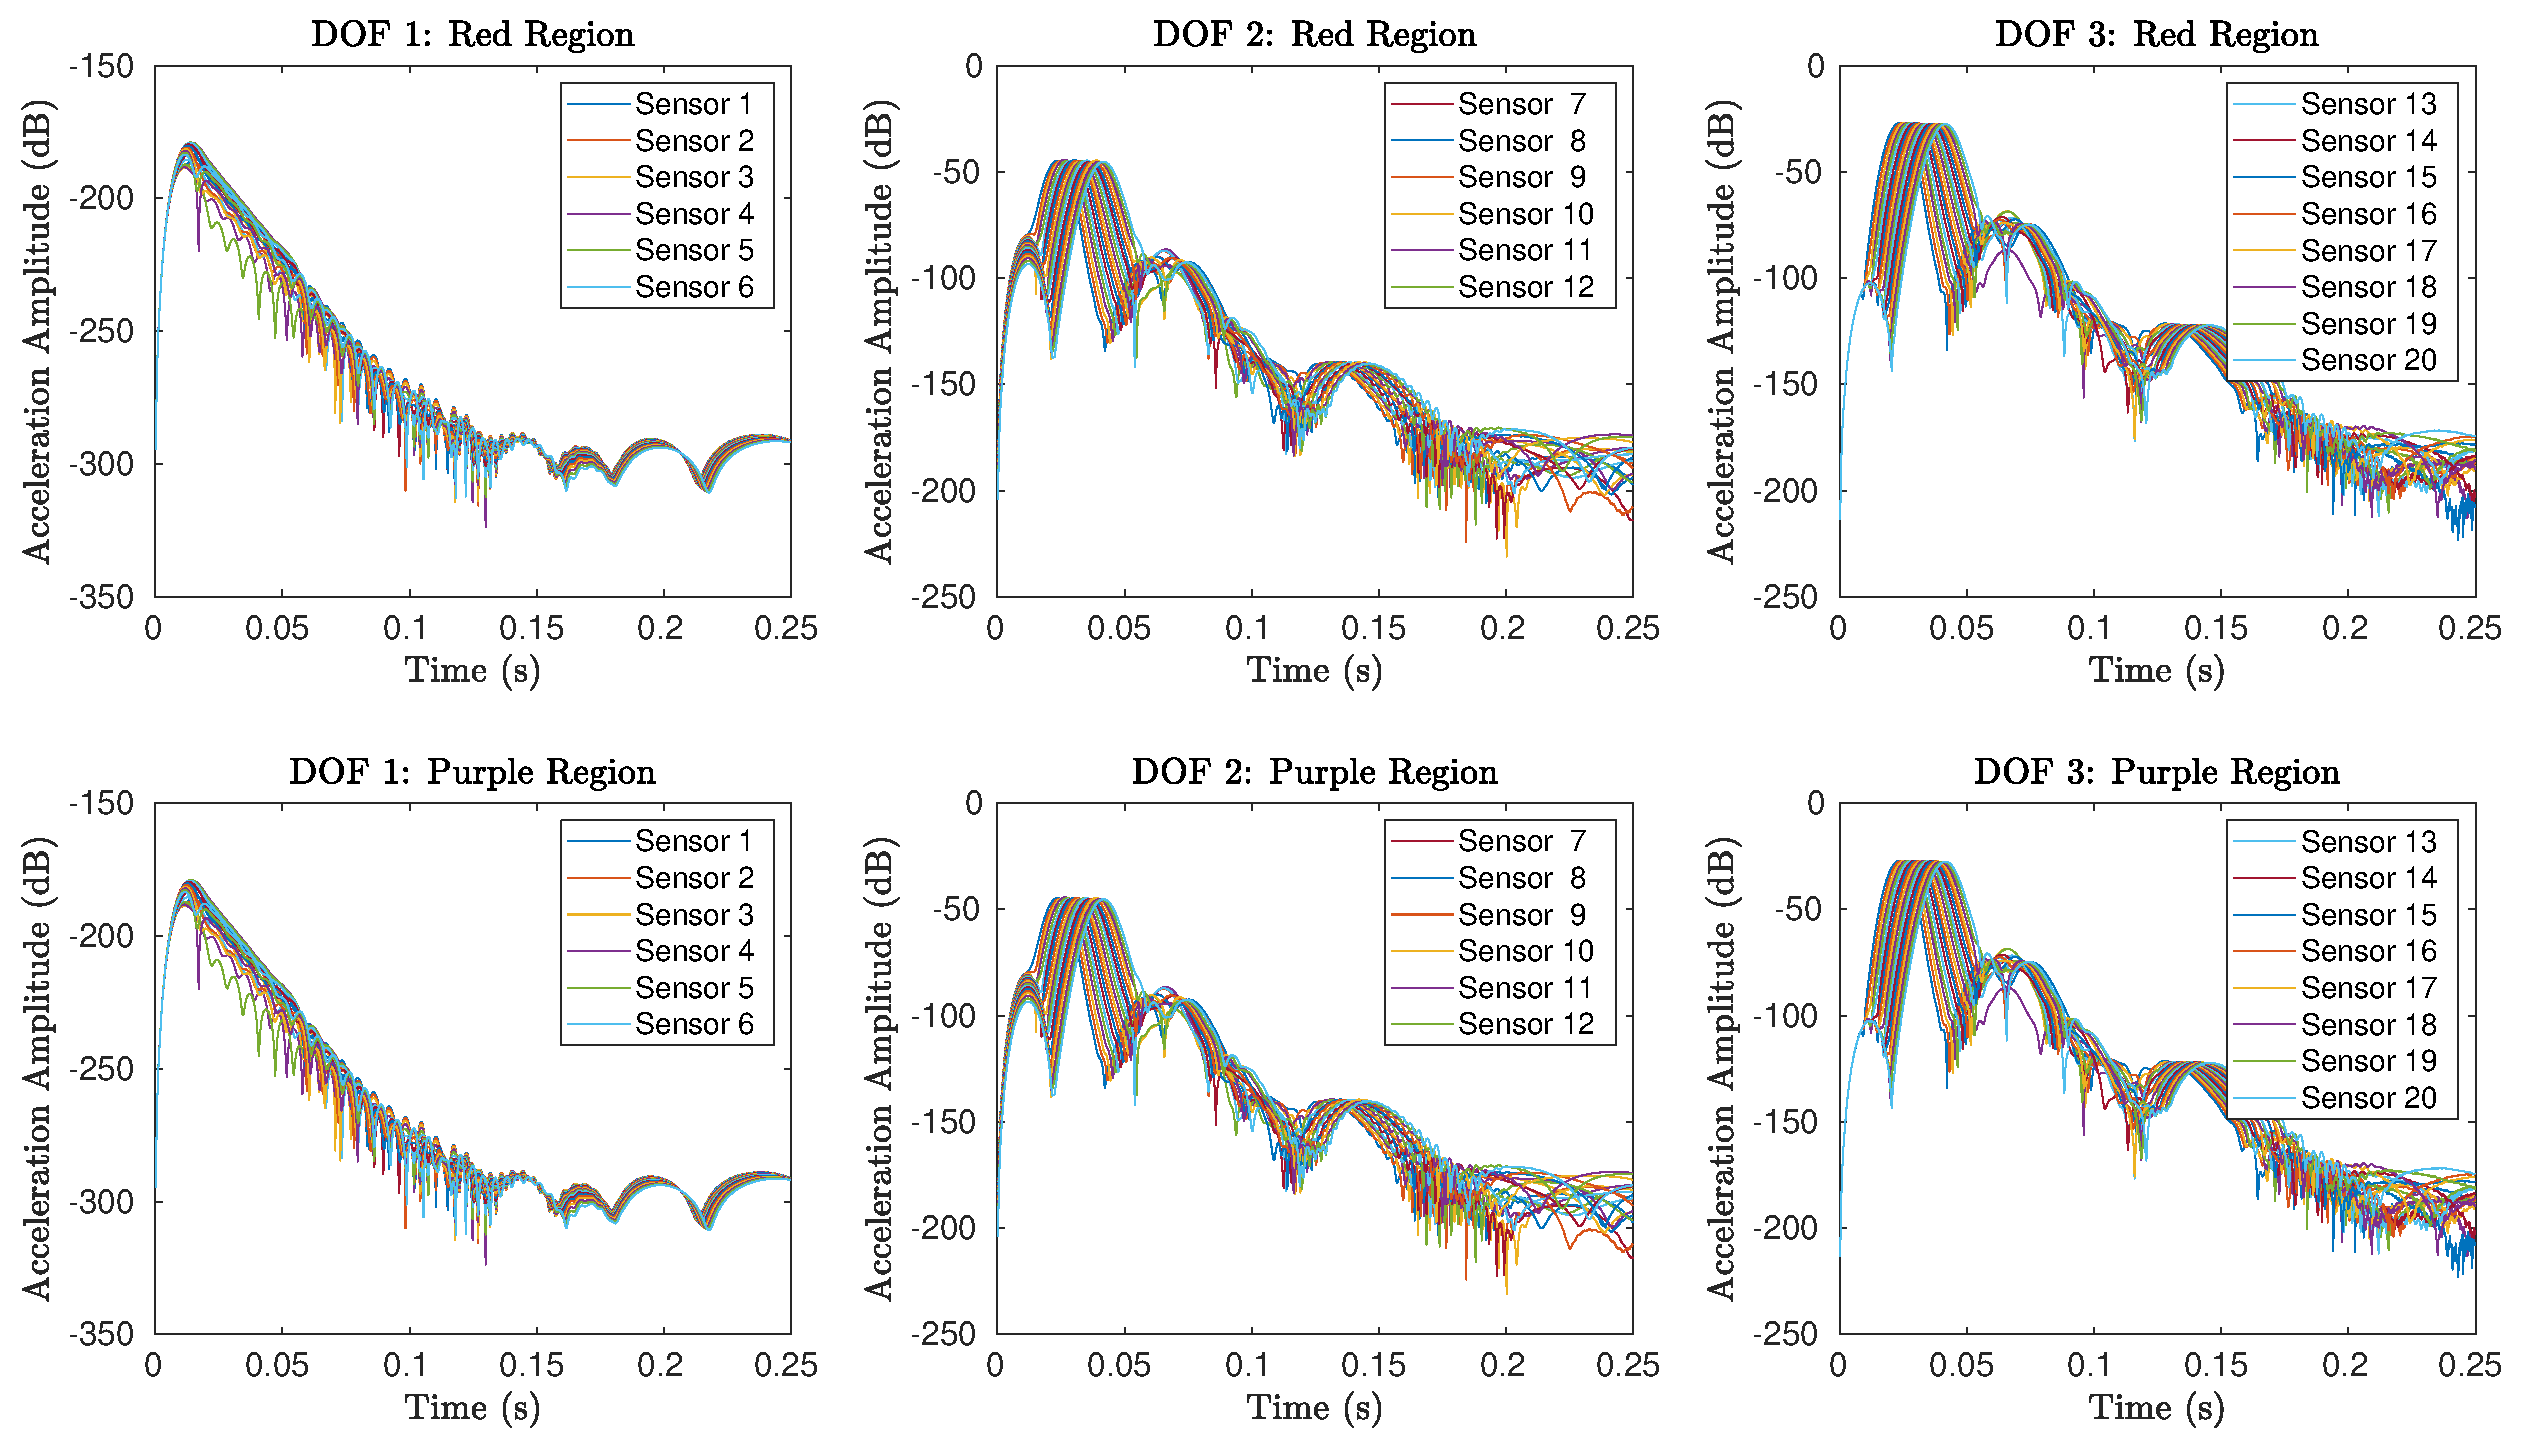
\includegraphics[width=0.7\linewidth]{../../PLANARMODEL/FIGS/FPULSERESP_samppuls}
    \end{figure}
    \pagebreak
  \item And here are the transmission coefficient estimates
    \begin{figure}
      \centering
      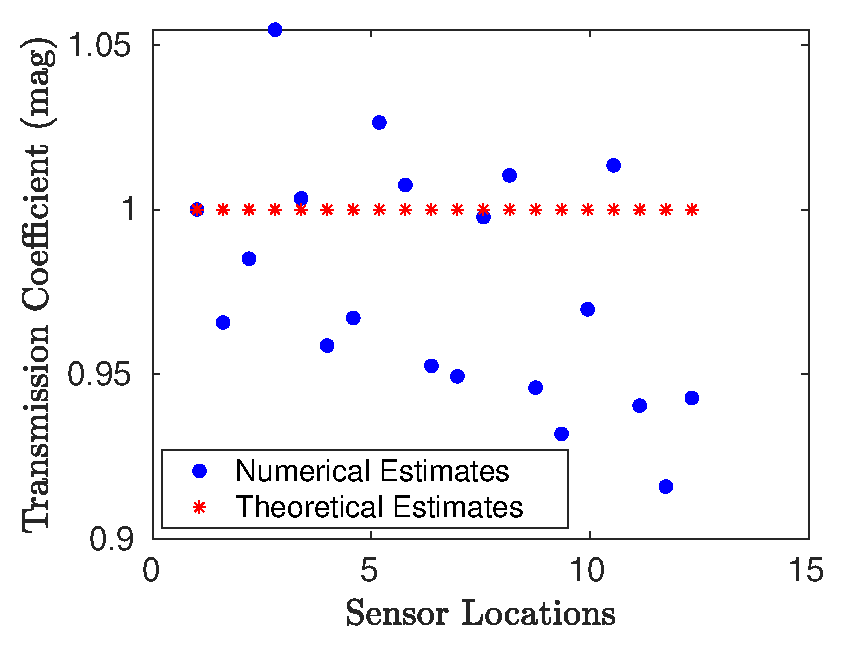
\includegraphics[width=0.5\linewidth]{../../PLANARMODEL/FIGS/FPULS_TMsamp}
    \end{figure}
  \item The theoretical estimates are
    $e^{-k_1(x_{dest}-x_{source})}$ (which assumes that the response
    only has the first kind of transverse waves). 
  \item However, as can be seen, the numerical estimates are nowhere
    near exact and I'm not sure \textbf{how to decompose a wave 
      solution into the different wave components.} 
  \item Further, at the location of forcing all the ``wave
    components'' get added up, thereby making detection even harder. 
  \end{itemize}
\end{frame}

\subsection{Approach 2: homogeneous Wave Propagation}
\label{sec:appr-2:-hom}

\begin{frame}[allowframebreaks]
  \frametitle{Numerical Wave-based Study Methodology}
  \framesubtitle{Approach 2: Homogeneous Wave Response}
  \begin{itemize}
  \item A more direct approach would be to solve this as an initial
    value problem with initial conditions specified as,
    {\footnotesize
      \begin{align*}
        u_x(x, 0) &= a_{\ell}^+ e^{-ik_\ell x} + a_{\ell}^- e^{ik_\ell
                    x}\\
        \begin{Bmatrix} u_y\\ \theta_z \end{Bmatrix} &= \begin{bmatrix}
          e^{-i(k_1x-\omega t)} & 
          e^{-(k_2x-i\omega t)} \\
          -(iP)e^{-i(k_1x-\omega t)} & -(N)
          e^{-(k_2x-i\omega t)} \end{bmatrix} \begin{Bmatrix} a_1^+\\
          a_2^+ \end{Bmatrix} + \begin{bmatrix} e^{i(k_1x+\omega t)} & 
          e^{(k_2x+i\omega t)}\\ (iP) e^{i(k_1x+\omega t)} & (N) e^{(k_2x+i\omega
            t)} \end{bmatrix} \begin{Bmatrix} a_1^-\\
          a_2^- \end{Bmatrix} 
      \end{align*}}
  \item Different choices of $a_{\ell,1,2}^\pm$ can be chosen and
    ``spatially windowed'' to obtain response
  \item Analysis of the response is, however, not very clear at the
    moment.
    \pagebreak
    Z\item I have written a code for this but have a few questions:
    \begin{enumerate}
    \item \textbf{How to localize the wave components?} Dr. Leamy had
      suggested using a Hann window spatially. While this works for
      the \emph{type 1} wave, it is not very obvious how this will
      work for the \textbf{type 2} wave, which is not harmonic in
      space.
    \item \textbf{How to decompose the transient solution from a
        finite element model into the different wave components?}
      I understand how to do this for wave components that are
      harmonic in space but since the non-harmonic component is also
      present, I'm not sure if we can do this with just Fourier
      methods. 
    \item \textbf{How to model amplitude dependence on the derived
        model?} When we say amplitude dependence, we need to determine
      how to choose an amplitude (or set of amplitudes) since we will
      have the interaction of 3 different kinds of waves for the
      nonlinear case (1 longitudinal and 2 transversal).
    \item I'm currently assuming that we're interested in obtaining a
      transmission matrix of the form
      \vspace{-0.25cm}
      $$ T(a_\ell^+, a_\ell^-, a_1^+, a_1^-, a_2^+, a_2^-) \in
      \mathbb{C}^{6\times 6}, $$
      such that
      \begin{align*}
        \begin{Bmatrix} b^+_\ell\\ b^-_\ell\\ b^+_1\\ b_1^-\\ b^+_2\\
          b_2^- \end{Bmatrix} = T(a_\ell^+, a_\ell^-, a_1^+, a_1^-,
        a_2^+, a_2^-) \begin{Bmatrix} a^+_\ell\\ a^-_\ell\\ a^+_1\\
          a_1^-\\ a^+_2\\ a_2^- \end{Bmatrix},
      \end{align*}
      where $a_{\ell,1,2}^\pm$ and $b_{\ell,1,2}^\pm$ represent the
      wave amplitudes ``before'' and ``after'' the joint is
      encountered. \textbf{Can this be simplified further?} I know for
      one that assumptions of symmetry \underline{can't be made} in
      the X direction (influence of $a_1^+$ on $b_1^+$ will be
      different from the influence of $a_1^-$ on $b_1^-$ (or other
      way)) due to the geometry of the BRB joint.
    \end{enumerate}
  \end{itemize}
\end{frame}

\section{Present Directions}
\label{sec:present-directions}

\begin{frame}[allowframebreaks]
  \frametitle{Present Directions}
  \begin{itemize}
  \item It may be a good starting step to derive the reflectance and
    transmittance matrices of a nonlinear element like the following
    \begin{figure}
      \centering
      \includegraphics[width=0.6\linewidth]{FIGS/SIMPMODS_1}
      
      \includegraphics[width=\linewidth]{FIGS/SIMPMODS_2}
    \end{figure}
  \item Some examples would be
    \begin{enumerate}
    \item The Bouc-Wen Model:
      \begin{align*}
        F(t) &= ak_{i}u(t)+(1-a)k_{i}z(t)\\
        {\dot {z}}(t) &= {\dot {u}}(t)\left\{A-\left[\beta \operatorname {sign} (z(t){\dot {u}}(t))+\gamma \right]|z(t)|^{n}\right\}.
      \end{align*}
    \item The Jenkins model:
      $$ dF(t) = \begin{cases} k_t du(t) & |F|<F_{slip}\\ F_{slip}
        sign(\frac{du}{dt}) & slip \end{cases} $$
    \end{enumerate}
  \item Here, $u$ denotes the \emph{relative displacement} experienced in the
    element and $F$ is the \emph{internal force} developed
  \end{itemize}
\end{frame}

\end{document}
%%% Local Variables:
%%% mode: latex
%%% TeX-master: t
%%% End:
